\section{VPN}

%Wie die Wireless Mesh Verbindungen zustande kommen geht aus dem
%Aufbau der Firmware bereits hervor. Wie jedoch die Knoten
%untereinander verbunden werden, soll der Vortrag in einem weiteren
%Abschnitt über das verwendete VPN zeigen. Dazu gehört auch die
%Aufteilung in Subnetze und die Verbindung der Gateways
%untereinander.

\begin{frame}{Allgemeines}
    \begin{itemize}
        \item Verwendetes VPN: fastd
        \item Layer-II Netz
        \item Wir nutzen keine Verschlüsselung (! :-O)
    \end{itemize}
    \begin{block}{fastd}
        % todo: was ist fastd ?
        There are no server and client roles defined by the
        protocol, this is just defined by the usage.
        \begin{itemize}
            \item Only one instance of the daemon is needed on each
                host to create a full mesh
            \item If no full mesh is established, a routing protocol
                is necessary to enable hosts that are not connected
                directly to reach each other
        \end{itemize}
    \end{block}
\end{frame}

\begin{frame}{Allgemeines}
    \begin{itemize}
        \item fastd Integration durch
        \begin{itemize}
            \item fastdstart.sh auf der Client-Seite
                \footnote{bsp/default/root\_file\_system/etc/fastdstart.sh.tpl}
            \item \$project\_\$hood\_fastd.sh auf der Server-Seite
                \footnote{auf den Gateways (!) Todo: befreien!}
            \item VPN-KeyXchange als Schlüsseltausch
                \footnote{\url{https://github.com/FreifunkFranken/VPNkeyXchange}}
        \end{itemize}
        \item Aufteilung in ,,hood''s:
        \begin{itemize}
            \item Stellt ein Layer-II Netz dar
            \item Ein Gateway kann mehrere Layer-II Netze bedienen
        \end{itemize}
    \end{itemize}
\end{frame}

\begin{frame}{Freifunk Hoods}
    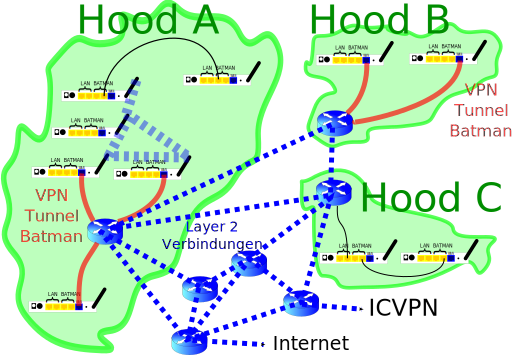
\includegraphics[width=\textwidth]{img/svg/freifunk_konzepte.pdf}

    Unser Freifunknetz ist in mehrere Layer-2 Inseln, die per Layer-3 miteinander verbunden sind,
    aufgeteilt. Die Hoods A und B in diesem Beispiel sind über unser VPN jeweise mit einem Router im
    Internet verbunden. Hood C hat einen lokalen Router, der direkt am LAN-Port hängt.
\end{frame}

\begin{frame}{\alt<1>{fastdstart.sh}{\$project\_\$hood\_fastd.sh}}
    \begin{itemize}
        \item \only<1>{Testet Internet-Connectivität}
        \item Legt fastd Konfiguration
            /etc/fastd/\$project\only<2>{.\$hood}/ \only<1>{im tmpfs} an:
            \footnote{\$project ist bei uns immer ,,fff''.}
            \begin{itemize}
                \item \$project.conf
                \item up.sh
                \item down.sh
                \item peers/
            \end{itemize}
        \item Erzeugt Pub/Priv-Keypaar
        \item Startet fastd
        \item Meldet sich beim VPN-KeyXchange an
        \item Lädt Liste mit Peers
        \item Refresht fastd
        \item \only<2>{Löscht verwaiste Peers}
    \end{itemize}
\end{frame}

\begin{frame}{VPN-KeyXchange}
    \only<1>{
        \begin{block}{HTTP Schnittstelle}
            \texttt{\tiny
                http://mastersword.de/\textasciitilde{}reddog/\$project/?mac=\$mac\&name=\$hostname\&port=\$port\&key=\$pubkey
            }
        \end{block}

        \begin{block}{Rückmeldung}
            \texttt{\tiny
                \#\#\#\#romauplink.conf\\
                \#name "romauplink";\\
                key "9a8ee8b797eed5d3b06778c47fe670987a0eda791ca557da56e6198be45f24c6";\\
                remote ipv4 "109.163.229.254" port 10000 float;\\[2ex]
                \#\#\#\#fff.conf\\
                \#name "fff";\\
                key "543ebc33b36210b10edf62fdb560e3ceac6c64b4ed9ad852f39954522934cd8a";\\
                remote ipv4 "192.168.30.23" port 10000 float;\\[2ex]
                \#\#\#\#90F652F45C34.conf\\
                \#name "ChamHH8Dachboden1";\\
                key "d0e4900fae535d189ef070a527dd00ce2688f3ff7f2b31c4f2846cb658b855fb";\\
                remote ipv4 "93.194.173.193" port 10000 float;\\
            }
        \end{block}
    }
    \only<2>{
        \begin{itemize}
            \item Knoten Identifizierung über MAC, alternativ über Name
            \item Jeweils pro hood:
            \begin{itemize}
                \item Clients bekommen eine Liste aller Gateways
                \item Gateways bekommen eine Liste aller Clients+Gateways
            \end{itemize}
        \end{itemize}
    }
    \only<3-7>{
        \begin{tabular}{|c|c|c|c|c|c|c|c|} \hline
            ID & mac & name & key & ip & port & gw & hood \\ \hline
            0 & & roup & abc & 254 & 10000 & true & 1 \\ \hline
            1 & & roup.fuerth & abd & 254 & 10001 & true & 2 \\ \hline
            2 & & nue1.fuerth & abe & 129 & 10001 & true & 2 \\ \hline
            3 & ab: & default-1 & abf & 1 & 10000 & false & 1 \\ \hline
            4 & cd: & default-2 & aca & 2 & 10000 & false & 1 \\ \hline
            5 & ef: & fuerth-1 & acb & 3 & 10000 & false & 2 \\ \hline
        \end{tabular}

        \only<4,5>{
            \begin{block}{?mac=ab:\&name=default-1\&..}
                \alt<4>{
                    SELECT ID,gw,hood FROM nodes WHERE mac = \$mac;\\
                    if (gw)\\
                    \hspace{1cm}SELECT * FROM nodes WHERE hood=\$hood\\
                    else\\
                    \hspace{1cm}SELECT * FROM nodes WHERE hood=\$hood \& gw=true\\
                }{
                    \begin{tabular}{|c|c|c|c|c|c|c|c|} \hline
                        ID & mac & name & key & ip & port & gw & hood \\ \hline
                        0 & & roup & abc & 254 & 10000 & true & 1 \\ \hline
                    \end{tabular}
                }
            \end{block}
        }
        \only<6,7>{
            \begin{block}{?mac=\&name=nue1.fuerth\&..}
                \alt<6>{
                    SELECT ID,gw,hood FROM nodes WHERE name = \$name;\\
                    if (gw)\\
                    \hspace{1cm}SELECT * FROM nodes WHERE hood=\$hood\\
                    else\\
                    \hspace{1cm}SELECT * FROM nodes WHERE hood=\$hood \& gw=true\\
                }{
                    \begin{tabular}{|c|c|c|c|c|c|c|c|} \hline
                        ID & mac & name & key & ip & port & gw & hood \\ \hline
                        1 & & roup.fuerth & abd & 254 & 10001 & true & 2 \\ \hline
                        2 & & nue1.fuerth & abe & 129 & 10001 & true & 2 \\ \hline
                        5 & ef: & fuerth-1 & acb & 3 & 10000 & false & 2 \\ \hline
                    \end{tabular}

                }
            \end{block}
        }
    }
\end{frame}
